\documentclass[usenames, dvipsnames]{beamer}

\useoutertheme{miniframes}
\beamertemplatenavigationsymbolsempty
\setbeamertemplate{footline}[frame number]

\usepackage[l2tabu, orthodox]{nag}

\usepackage[utf8]{inputenc}
\usepackage[T1]{fontenc}

\usepackage[english]{babel}

\usepackage{amsmath}
\usepackage{amssymb}
\usepackage{amsthm}
\usepackage{mathtools}
\usepackage{physics}
\usepackage{centernot}

\usepackage{csquotes}
\usepackage{lmodern}
\usepackage{microtype}
\usepackage{framed}

\usepackage{parskip}

\usepackage{tikz}

\usepackage{listings}

\MakeOuterQuote{"}

    \makeatletter
    \let\beamer@writeslidentry@miniframeson=\beamer@writeslidentry
    \def\beamer@writeslidentry@miniframesoff{%
      \expandafter\beamer@ifempty\expandafter{\beamer@framestartpage}{}% does not happen normally
      {%else
        % removed \addtocontents commands
        \clearpage\beamer@notesactions%
      }
    }
    \newcommand*{\miniframeson}{\let\beamer@writeslidentry=\beamer@writeslidentry@miniframeson}
    \newcommand*{\miniframesoff}{\let\beamer@writeslidentry=\beamer@writeslidentry@miniframesoff}
    \beamer@compresstrue
    \makeatother

\lstset{language=C++,
	basicstyle=\ttfamily\footnotesize,
	tabsize=4,
	breaklines=true}

\title{Windows GUI}
\subtitle{Proseminar Windows Internals}
\author{Markus Himmel}

\newcommand{\li}{
	\node at (0, 0) {};
	\node at (12, 10.5) {};
	\draw[thick] (0, 5) -- (12, 5);
	\node[anchor=south east] at (12, 5) { \small User };
	\node[anchor=north east] at (12, 5) { \small Kernel };
}

\newcommand{\apps}{
	\draw (0, 9.5) rectangle node (apps) { Applications } ++(10.5, 1);
}

\newcommand{\user}{
	\draw (0, 5.5) rectangle node { user32 } ++(1.5, 1);
	\draw (0.75, 6.5) -- ++(0, 3);
}

\newcommand{\wink}{
	\draw (0, 3.5) rectangle node { \texttt{win32k.sys} } ++(10.5, 1);
	\draw (0.75, 4.5) -- ++(0, 1);
	\draw (0, 0.25) rectangle node[align=center,text width=2.5cm] { Kernel-mode I/O Manager } ++(3, 2.25);
	\draw[dashed,color=black!60] (0, 3) -- (12, 3);
	\draw (1.5, 2.5) -- ++(0, 1);
}

\newcommand{\drawgdi} {
	\draw (1.75, 5.5) rectangle node (gdi32) { gdi32 } ++(1.5, 1);
	\draw (2.5, 6.5) -- ++(0, 3);
	\draw (2.5, 4.5) -- ++(0, 1);
	\draw (0.2, 3.7) rectangle node { GDI } ++(1, 0.6);
	\draw (3.5, 0.25) rectangle node { Kernel-mode Display Driver } ++(7, 1);
	\draw (3.5, 1.5) rectangle node { Canonical Display Driver } ++(7, 1);
	\draw (7, 2.5) -- ++(0, 1);
	\draw (7, 1.25) -- ++(0, 0.25);
}

\newcommand{\drawing}{
	\draw (3.75, 5.5) rectangle node { DirectX } ++(2, 1);
	\draw (3.75, 6.75) rectangle node { milcore } ++(2, 1);

	\draw (6, 5.5) rectangle node { User-mode D3D Driver } ++(4.5, 1);
	\draw (3.75, 8) rectangle node { Avalon } ++(2, 1);

	\draw (3.75, 6) -| ++(-0.25, 3.5);
	\draw (4.75, 9) -- ++(0, 0.5);

	\draw (4.75, 7.75) -- ++(0, 0.25);
	\draw (4.75, 6.5) -- ++(0, 0.25);
	\draw (5.75, 6) -- ++(0.25, 0);

}

\newcommand{\dwm}{
	\draw (6, 8) rectangle node { DWM } ++(2, 1);
	\draw (7, 9) -- ++(0, 0.5);
	\draw (5.75, 7.25) -| ++(1.25, 0.75);
}

\newcommand{\arch}[1]{
	\miniframesoff
	\begin{frame}{Architecture of the Windows GUI}
		\begin{tikzpicture}[xscale=0.95, yscale=0.7]
			#1
		\end{tikzpicture}
	\end{frame}
	\miniframeson
}

\begin{document}
	\maketitle
	\section{Preliminaries}
	\setcounter{subsection}{1}
	\begin{frame}{Graphical User Interfaces}
		\begin{itemize}
			\item "Interface to an electronic device using graphical icons and
				visual indicators"
			\item Often (?) more intuitive and better methaphors than command-line interface
			\item Prevalent paradigm for personal computers: windows, icons, menus, pointer (WIMP)
			\item Core focus for this presentation: Responsiveness!
				\begin{itemize}
					\item 100ms for a reaction to feel instantaneous
					\item Humans can easily distinguish between refresh rates of 30Hz and 60Hz
				\end{itemize}
		\end{itemize}
	\end{frame}

	\section{Win32 GUI Applications}
	\setcounter{subsection}{1}
	\arch{\li\apps}
	\begin{frame}{Windows and Window Handles}
		\begin{itemize}
			\item Fundamental building block: Window
			\item Controls are also windows
				\begin{itemize}
					\item Parent pointer $\leadsto$ hierarchy
				\end{itemize}
			\item Appearance and behavior determined by
				\emph{Window Classes}
			\item After registering window class, application can create window
				of that class and receives \emph{Window Handle} (\texttt{HWND})
			\item Functions/system calls that query or manipulate window
				are passed \texttt{HWND}
		\end{itemize}
	\end{frame}


	\begin{frame}[fragile]{Window Messages and Procedures (1)}
		\begin{itemize}
			\item Main entry point of Win32 GUI app must be message
				loop
			\item Messages handed over to \textit{Window Procedure}
		\end{itemize}
		\hfill
		\begin{lstlisting}
int WINAPI wWinMain(...)
	// Set up and show window

	MSG msg = { };
	while (GetMessage(&msg, NULL, 0, 0))
	{
		TranslateMessage(&msg);
		DispatchMessage(&msg);
	}
}
		\end{lstlisting}
	\end{frame}
	\begin{frame}[fragile]{Window Messages and Procedures (2)}
		\begin{itemize}
			\item Window Procedure handles messages. Examples:
				\begin{itemize}
					\item User input
					\item Requests to draw
					\item Application exit
				\end{itemize}
		\end{itemize}
		\begin{lstlisting}
LRESULT CALLBACK WindowProc(HWND hwnd, UINT uMsg, WPARAM wParam, LPARAM lParam)
{
	switch (uMsg)
	{
	case WM_PAINT:
		{
			// Extract parameters and call handler
		}
		break;
	}
	return DefWindowProc(hwnd, uMsg, wParam, lParam);
}
		\end{lstlisting}
	\end{frame}

	\arch{\li\apps\user}
	\begin{frame}{\texttt{win32k.sys}}
		\begin{itemize}
			\item Kernel component that manages GUI applications
			\item Keeps track of all active GUI threads
				\begin{itemize}
					\item Threads promoted when first calling into \texttt{win32k.sys}
					\item For instance via \texttt{user32.dll} when calling \texttt{CreateWindowEx}
					\item Bigger kernel stack, \texttt{win32k} data structures
				\end{itemize}
			\item Maintains \emph{Raw Input Thread}: Polls peripherals,
				posts messages to correct window
			\item NT 3.51: User-mode
			\item Moved primarily for performance reasons
				\begin{itemize}
					\item High frequency and bandwidth of driver communication
					\item \textit{Modified microkernel}
					\item Interface and architecture unchanged $\leadsto$ \textit{Huge} security problems
				\end{itemize}
		\end{itemize}
	\end{frame}

	\arch{\li\apps\user\wink}


	\section{Drawing the GUI to the screen}
	\setcounter{subsection}{1}

	\begin{frame}{Windows GUI Drawing APIs (1)}
		\begin{itemize}
			\item Graphics Device Interface (GDI)
				\begin{itemize}
					\item Classic Windows API for GUI applications
					\item Rendered by CPU to system memory
						\begin{itemize}
							\item Hardware-accelerated in \textit{some} Windows versions
						\end{itemize}
					\item Not used for new applications
					\item User-mode components in \texttt{gdi32.dll}
					\item Kernel-mode support in \texttt{win32k.sys}
						\begin{itemize}
							\item Talks to graphics driver
						\end{itemize}
				\end{itemize}
		\end{itemize}
	\end{frame}

	\arch{\li\apps\user\wink\drawgdi}

	\begin{frame}{Windows GUI Drawing APIs (2)}
		\begin{itemize}
			\item DirectX
				\begin{itemize}
					\item Actually multiple APIs called Direct3D, DirectDraw, \ldots
					\item Runs on GPU, uses video memory
					\item Originally: game programming
					\item Now: hardware-accelerated rendering of regular GUI applications
				\end{itemize}
			\item Avalon a.k.a. Windows Presentation Foundation (WPF)
				\begin{itemize}
					\item Example of a higher-level GUI framework
					\item Designed for the CLR
					\item Renders using DirectX in a native component called \texttt{milcore.dll}
						(stay tuned)
				\end{itemize}
		\end{itemize}
	\end{frame}

	\arch{\li\apps\user\wink\drawgdi\drawing}

	\begin{frame}{The Desktop Window Manager (DWM)}
		\begin{itemize}
			\item \textit{Compositing} Window Manager introduced in Longhorn
			\item Benefits:
				\begin{itemize}
					\item Elimination of tears and trails
					\item Visual Effects: Transparency/\enquote{Glass}, Previews, Windows Flip
				\end{itemize}
			\item Implemented as a full screen DirectX application
				\item Applications render into one (DirectX) or two (GDI) off-screen
					buffers
				\item DWM manages repaint requests and stitches together final desktop
				\item Little more than a typical WPF app---both use user-space \texttt{milcore.dll} to
					perform rendering
		\end{itemize}%
		\begin{tikzpicture}[remember picture,overlay]%
		\only<2>{%
			\node[xshift=20mm,yshift=-12mm,anchor=north west] at (current page.north west){%
			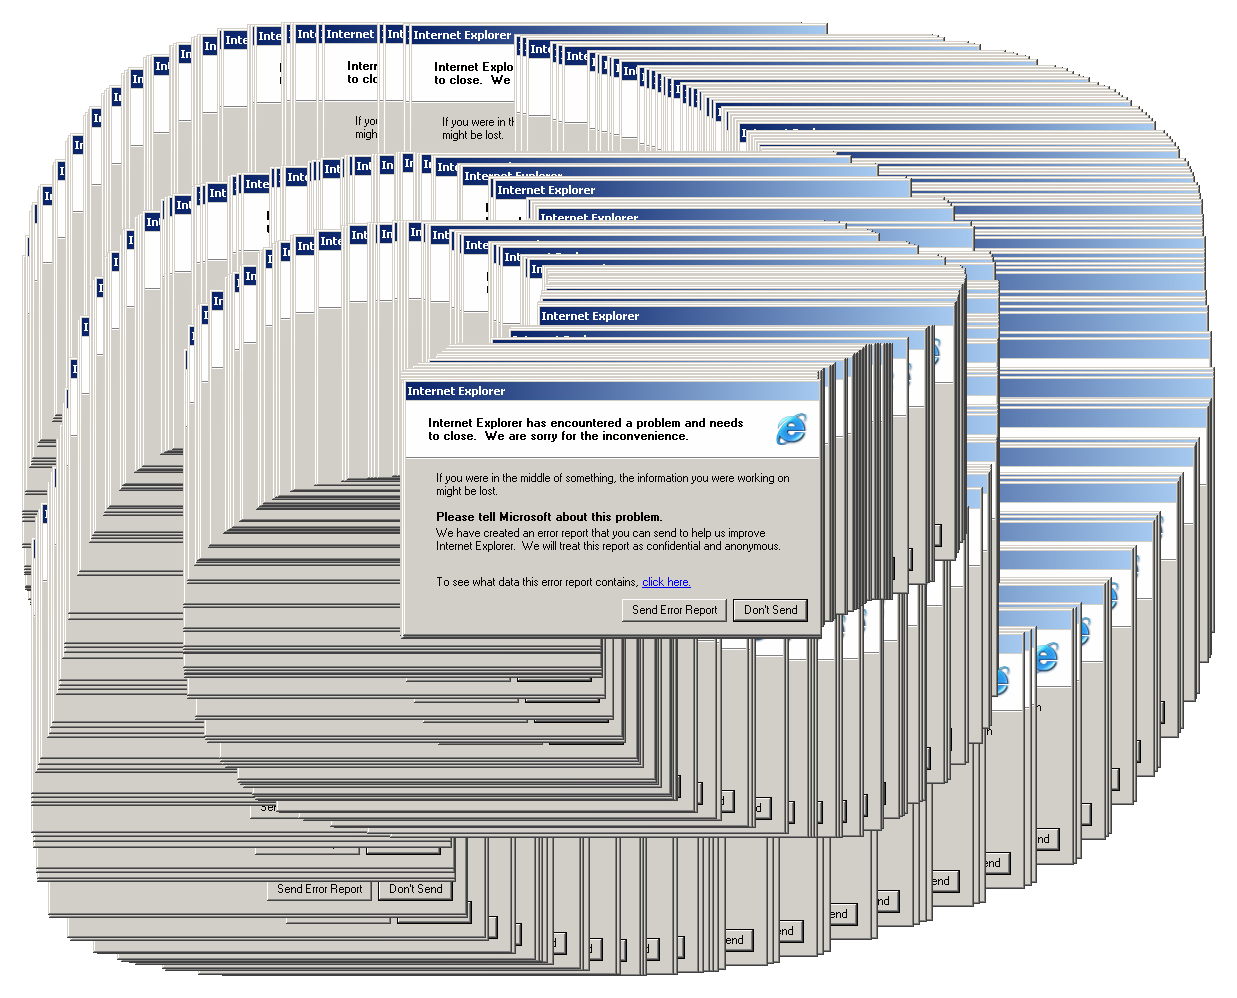
\includegraphics[width=8cm]{trail}};}
		\end{tikzpicture}%
		\only<3>{}
	\end{frame}


	\begin{frame}{The Windows Display Driver Model: Benefits}
		\begin{itemize}
			\item Problem: DWM as described is painfully slow
				\begin{itemize}
					\item DirectX: exclusive control of GPU
					\item DWM concurrent with other DirectX apps, wildly varying memory
						requirements
					\item Countless copies of buffers
				\end{itemize}
			\item WDDM: Framework for Windows display drivers
			\item Features key to DWM performance:
				\begin{itemize}
					\item Virtualization of video memory
					\item Interruptability of the GPU
					\item DirectX surface sharing
				\end{itemize}
		\end{itemize}
	\end{frame}

	\arch{\li\apps\user\wink\drawgdi\drawing\dwm}
\end{document}
